% -------------------------------
% Plantilla del TFG en la ESIIAB-UCLM. Versión 0.0 (Preliminar)
%
% Luis de la Ossa
% 
% Compilar con XeLaTeX 
% -------------------------------
\documentclass[12pt, a4paper]{book}

% -------------------------------
% Información y opciones del documento. Debe editarse.
% -------------------------------
% -------------------------------
% Plantilla del TFG en la ESIIAB-UCLM. Versión 0.0 (Preliminar)
%
% Luis de la Ossa
% 
% Compilar con XeLaTeX 
% -------------------------------


% -------------------------------
% Comandos comunes
% -------------------------------
\newcommand{\uclm}{Universidad de Castilla-La Mancha\,}
\newcommand{\dsi}{Departamento de Sistemas Informáticos\,}
\newcommand{\esii}{Escuela Superior de Ingeniería Informática de Albacete\,}
\newcommand{\iiia}{Instituto de Investigación en Informática de Albacete\,}


% -------------------------------
% Comandos específicos
% -------------------------------
\newcommand{\autor}{Fernando Lozano Catalán\,}
\newcommand{\titulo}{Desarrollo de una Aplicación para la Automatización de Procesos en Empresas Pequeñas\,}
\newcommand{\director}{José Antonio Gallud Lázaro\,}
\newcommand{\codirector}{Felipe Costa Tébar\,}
\newcommand{\fecha}{Mayo, 2025\,}
 \newcommand{\espec}{Tecnología Específica de Ingeniería del Software\,} 







% -------------------------------
% Configuración del documento, paquetes, etc. 
% -------------------------------
\input{include/configuracion}

% Documento
\begin{document}

% -------------------------------
% Portada y título
% -------------------------------
% Fuente  de la portada
% \setmainfont[Ligatures={NoRequired,NoCommon,NoContextual}]{Calibri}
\input{elements/portada}

% -------------------------------
% Fuente del documento.
% -------------------------------
% La fuente recomendada es Calibri, pero no está instalada en overleaf:
%\setmainfont[Ligatures={NoRequired,NoCommon,NoContextual}]{Calibri}

% Para utilizarla aquí, son necesarios los archivos .ttf correspondientes:
%\setmainfont[
%			BoldFont=Calibrib.ttf,
%			ItalicFont=Calibrii.ttf,
%			BoldItalicFont=Calibriz.ttf
%		]{Calibri.ttf}

% Por defecto, utiliza una fuente instalada en overleaf. 
% Éstas son algunas que van bien con la plantilla:
%\setmainfont{Alegreya Sans} 
\setmainfont{Carlito}
%\setmainfont{PT Sans}
%\setmainfont{Source Sans Pro}

% -------------------------------
% Preámbulo
% -------------------------------
\frontmatter 
% -------------------------------
% Plantilla del TFG en la ESIIAB-UCLM. Versión 0.0 (Preliminar)
%
% Luis de la Ossa
% 
% Compilar con XeLaTeX 
% -------------------------------


% -------------------------------
% Segunda portada
% -------------------------------
\cleardoublepage
\setcounter{page}{1} \null

\begin{textblock*}{3cm}(3cm,2cm) 
\begin{flushleft}

\includegraphics[height=2cm]{figs/logouclm.png}
\end{flushleft}
\end{textblock*}


\begin{textblock*}{2.5cm}(15.95cm,2.45cm) 
\begin{flushright}

\includegraphics[height=1.4cm]{figs/euroinf.jpg}
\end{flushright}
\end{textblock*}

\begin{textblock*}{2cm}(14cm,2cm)  % Corrige la posición porque la imagen tiene margen
\begin{flushright}

\includegraphics[height=2cm]{figs/logoesii.png}
\end{flushright}
\end{textblock*}



\begin{textblock*}{\textwidth}(3cm,8cm) 
\begin{center}\doublespacing 
{\fontsize{18pt}{4pt}\selectfont \bft{TRABAJO FIN DE GRADO}}

\medskip
{\fontsize{18pt}{4pt}\selectfont Grado en Ingeniería Informática}

\medskip
{\fontsize{16pt}{4pt}\selectfont \espec}
\end{center}
\end{textblock*}


\begin{textblock*}{\textwidth}(3cm,14cm) 
\begin{center}\setstretch{2}
{\fontsize{22pt}{4pt}\selectfont \bft{\titulo}}
\end{center}
\end{textblock*}


\begin{textblock*}{\textwidth}(3cm,20.5cm) 
\begin{flushleft}\doublespacing
{\fontsize{14pt}{4pt}\selectfont \bft{Autor:} \autor}

{\fontsize{14pt}{4pt}\selectfont \bft{Tutor:} \director}

{\fontsize{14pt}{4pt}\selectfont \bft{Co-Tutor:} \codirector}
\end{flushleft}
\end{textblock*}


\begin{textblock*}{\linewidth}(3cm,25cm) 
\begin{flushright}
{\fontsize{14pt}{4pt}\selectfont \fecha}
\end{flushright}
\end{textblock*}


% -------------------------------
% Dedicatoria
% -------------------------------
\cleardoublepage
\thispagestyle{empty}

\vspace*{9cm}  
\begin{flushright} \em 
Aquí va la dedicatoria que cada cual \\ 
quiera escribir. El ancho se controla \\ 
manualmente
\end{flushright}


% -------------------------------
% Declaración de autoría
% -------------------------------
\cleardoublepage
\thispagestyle{plain}
\begin{center}
\Large{\bft{Declaración de autoría}}
\end{center}
\vskip1cm

Yo, \autor, con DNI 49426228X, declaro que soy el único autor del trabajo fin de grado titulado ``\titulo'', que el citado trabajo no infringe las leyes en vigor sobre propiedad intelectual, y que todo el material no original contenido en dicho trabajo está apropiadamente atribuido a sus legítimos autores.

\vspace*{2cm}
\begin{center}
Albacete, a \quad \ldots \quad de \quad \ldots \quad de 20 \ldots

\vskip3cm

Fdo.: \autor
\end{center}


% -------------------------------
% Resumen
% -------------------------------
\cleardoublepage
\thispagestyle{plain}
\begin{center}
\Large{\bft{Resumen}}
\end{center}
\vskip1cm
Este Trabajo de Fin de Grado presenta el desarrollo de una aplicación orientada a facilitar el funcionamiento diario de pequeñas y medianas empresas que cuentan con procesos repetitivos y carecen de gestores de contenidos avanzados. La aplicación permitirá al usuario registrar tanto una empresa como a un particular. Durante el desarrollo del TFG, se analizarán las necesidades de automatización y se seleccionará un conjunto de procesos. Por último, la aplicación ofrecerá un tablero Kanban que facilitará la organización y coordinación entre los usuarios, permitiéndoles crear ítems, gestionar tareas y visualizar su estado de forma clara y estructurada.

% -------------------------------
% Agradecimientos
% -------------------------------
\cleardoublepage
\thispagestyle{plain}
\begin{center}
\Large{\bft{Agradecimientos}}
\end{center}
\vskip1cm

\lipsum[1]

% -------------------------------
% Índices y tablas
% -------------------------------
\tableofcontents	% Índice
\listoffigures		% Índice de figuras
\listoftables		% Índice de tablas
\listofalgorithms   % Índice de algoritmos (comentar si no los hay)
\listofcodes	    % Índice de códigos (comentar si no los hay)
\cleardoublepage

% -------------------------------
% Documento
% -------------------------------
\mainmatter
% Estilo de página
\pagestyle{fancy}

% Introducción
\chapter{Introducción}
\section{Motivacion}
La digitalización en las pequeñas y medianas empresas (pymes) representa un desafío crítico en la actualidad, donde la tecnología actúa como el motor fundamental para la competitividad y la eficiencia. No obstante, existe una brecha significativamente grande entre las necesidades digitales de la empresa y la realidad tecnológica de las pymes locales, las cuales arrastran una deuda técnica que limita su crecimiento y capacidad de respuesta.

El origen de este proyecto parte de la experiencia directa con una pyme cercana al autor, en la cual se han podido observar las carencias producidas por esta deuda técnica. A lo largo de un extenso periodo de observación en esta pyme y varias cercanas del sector, se ha podido comprobar cómo esta falta de digitalización deriva en un uso ineficiente de herramientas muy básicas, como hojas de cálculo, para tareas que requieren estructuras de datos más robustas y centralizadas. Esta realidad provoca la aparición de procesos manuales repetitivos, silos de información sin conectar y una dependencia excesiva de comunicaciones, como llamadas telefónicas o reuniones virtuales constantes, para cubrir la falta de un sistema de autogestión. Este problema no solo empeora la productividad de la empresa, sino que se provoca un aumento innecesario de la carga de trabajo y del estrés del personal.

En este contexto, el presente Trabajo de Fin de Grado surge de la identificación de estos patrones de ineficiencia y de la voluntad de aplicar los conocimientos en análisis de procesos y desarrollo de software adquiridos durante la carrera. El proyecto tratara de crear una solución software que busca transformar esta gestión fragmentada en un ecosistema automatizado y coherente.

En resumen, este trabajo se basa en el desarrollo de una aplicación orientada a la gestión y automatización de procesos operativos, permitiendo a las pymes optimizar su funcionamiento diario y mejorar la coordinación entre usuarios mediante herramientas de gestión visual.  Con el fin de alcanzar estos objetivos y garantizar una respuesta adaptativa a las necesidades detectadas, se utiliza una metodología ágil para la gestión de la documentación y el desarrollo de las tareas.
\section{Objetivos}

El objetivo principal de este Trabajo de Fin de Grado es el diseño e implementación de una plataforma de software centralizada que integre un motor de automatización de flujos de trabajo y herramientas de gestión visual. En particular, se pretende desarrollar una solución que permita a las pequeñas y medianas empresas (pymes) optimizar sus procesos operativos repetitivos mediante n8n, a la vez que se facilita la autogestión de tareas y recursos a través de un tablero Kanban y un sistema de planificación integrados.

El cumplimiento del objetivo principal se articula a través de los siguientes objetivos específicos:

\begin{itemize}
    \item[\textbf{OBJ-1}] \textbf{Estudio del contexto y análisis de requisitos:} Realizar un estudio sobre la deuda tecnológica en las pymes de ámbito local, identificando los procesos manuales más críticos y analizando aplicaciones de automatización e integración existentes en el mercado.
    
    \item[\textbf{OBJ-2}] \textbf{Análisis y selección de tecnologías:} Evaluar y seleccionar las tecnologías más adecuadas para la implementación de una arquitectura robusta, cconsiderando el uso de motores de automatización, bases de datos relacionales y entornos de desarrollo web modernos.
    
    \item[\textbf{OBJ-3}] \textbf{Adopción de una metodología ágil:} Aplicar un enfoque de desarrollo ágil basado en iteraciones (\textit{sprints}) que permita la gestión del cambio y la incorporación progresiva de funcionalidades.
    
    \item[\textbf{OBJ-4}] \textbf{Implementación de la solución integral:} Desarrollar el prototipo funcional aplicando prácticas sólidas de Ingeniería del Software (patrones de diseño, modularidad e interfaces de conexión) para garantizar un sistema eficiente, escalable y de alta calidad.
    
    \item[\textbf{OBJ-5}] \textbf{Evaluación y validación de la calidad:} Realizar pruebas de integración entre la aplicación centralizada y el motor de automatización para asegurar la integridad de los datos y la correcta ejecución de los flujos de trabajo diseñados.
\end{itemize}

\section{Competencias de la Intensificación}

Las competencias de la intensificación de Ingeniería del Software que se pretenden cubrir en este Trabajo de Fin de Grado son las siguientes:

\begin{itemize}
    \item[\textbf{IS-1}] \textbf{Capacidad para desarrollar, mantener y evaluar servicios y sistemas software} que satisfagan todos los requisitos del usuario y se comporten de forma fiable y eficiente, sean asequibles de desarrollar y mantener y cumplan normas de calidad, aplicando las teorías, principios, métodos y prácticas de la Ingeniería del Software.
    
    \item[\textbf{IS-3}] \textbf{Capacidad de dar solución a problemas de integración} en función de las estrategias y tecnologías disponibles.
    
    \item[\textbf{IS-4}] \textbf{Capacidad de identificar y analizar problemas y diseñar, desarrollar, implementar, verificar y documentar soluciones software} sobre la base de un conocimiento adecuado de las teorías, modelos y técnicas actuales.
    
    \item[\textbf{IS-5}] \textbf{Capacidad de identificar, evaluar y gestionar los riesgos potenciales asociados} que pudieran presentarse durante el ciclo de vida del desarrollo.
\end{itemize}
\section{Estructura del Proyecto}
En este apartado se expone la organización que seguirá el presente Trabajo de Fin de Grado, proporcionando una breve descripción del contenido de cada uno de los capítulos que componen la memoria.

\begin{itemize}
    \item \textbf{Capítulo 1. Introducción:} Se introduce el contexto del trabajo y se explica el porqué de su realización. Asimismo, se definen el objetivo principal y los objetivos secundarios, finalizando con la descripción de las competencias de la intensificación que se pretenden cubrir.
    
    \item \textbf{Capítulo 2. Antecedentes:} Se detalla el contexto del trabajo planteando un enfoque que va desde lo más general a lo particular. En este bloque se profundiza en la tecnología relevante para el sector y se realiza un estudio de aplicaciones similares existentes en el mercado.
    
    \item \textbf{Capítulo 3. Propuesta de Solución, Metodología y Herramientas:} Se plantea formalmente la idea antes de su desarrollo y se define la metodología de trabajo a seguir. Además, se enumeran las herramientas utilizadas para la gestión, documentación y desarrollo del software.
    
    \item \textbf{Capítulo 4. Descripción de la Aplicación:} Constituye el núcleo técnico del trabajo, donde se detallan los requisitos del sistema y la arquitectura diseñada. Incluye un resumen del proceso de desarrollo y la descripción funcional de la aplicación resultante.
    
    \item \textbf{Capítulo 5. Evaluación:} Se describe el proceso de validación del sistema a través de diferentes niveles, como la usabilidad y la satisfacción del usuario. Se exponen los resultados obtenidos y su correspondiente discusión.
    
    \item \textbf{Capítulo 6. Conclusiones y Trabajo Futuro:} Se resume el grado de cumplimiento de los objetivos y competencias planteados inicialmente. Para finalizar, se proponen ideas clave para la evolución futura del proyecto.
\end{itemize}
Complementariamente, la memoria incluye un apartado de \textbf{Bibliografía} con todas las referencias utilizadas y una serie de \textbf{Anexos} destinados a detallar el desarrollo del proyecto por sprints y a facilitar material adicional como el acceso a repositorios o prototipos.

 

% Algunos elementos
\chapter{Antecedentes}
En este capítulo se presenta el contexto de las pequeñas empresas del sector de la construcción y las instalaciones de climatización. Se realizará una investigación que partira desde lo más general de la obra pública y la estructura de las PYMES del sector, hasta llegar al análisis de los procesos de gestión internos que presentan mayores ineficiencias. Asimismo, se examinará el estado actual de la tecnología en el sector, identificando las limitaciones de las herramientas tradicionales y evaluando las soluciones actuales.
\section{Ámbito de la obra pública en el sector aeroportuario}
La empresa se centra en el ámbito concreta de la obra publica aeroportuaria, el cual es un entorno altamente regulado, donde la carga administrativa suele superar la capacidad técnica de las pequeñas empresas. En esta sección se analizarán los mecanismos de licitación pública y los requisitos específicos de seguridad que condicionan la operativa diaria en infraestructuras críticas, basándose en el marco normativo vigente \cite{SEDIA2026}.
Las empresas que operan en el sector público deben participar en procesos de \textbf{licitación} convocados por diversos organismos e instituciones (ayuntamientos, ministerios, entes públicos, etc.). Este proceso sigue una estructura específica que marca el inicio de cualquier proyecto.En la figura \ref{fig:proceso_licitacion} podemos observar un diagrama de flujo, donde podemos ver las multiples fases del proceso que van desde el analisis de la licitación hasta la adjudicación de esta.
\newpage
\begin{figure}[h]
    \centering
    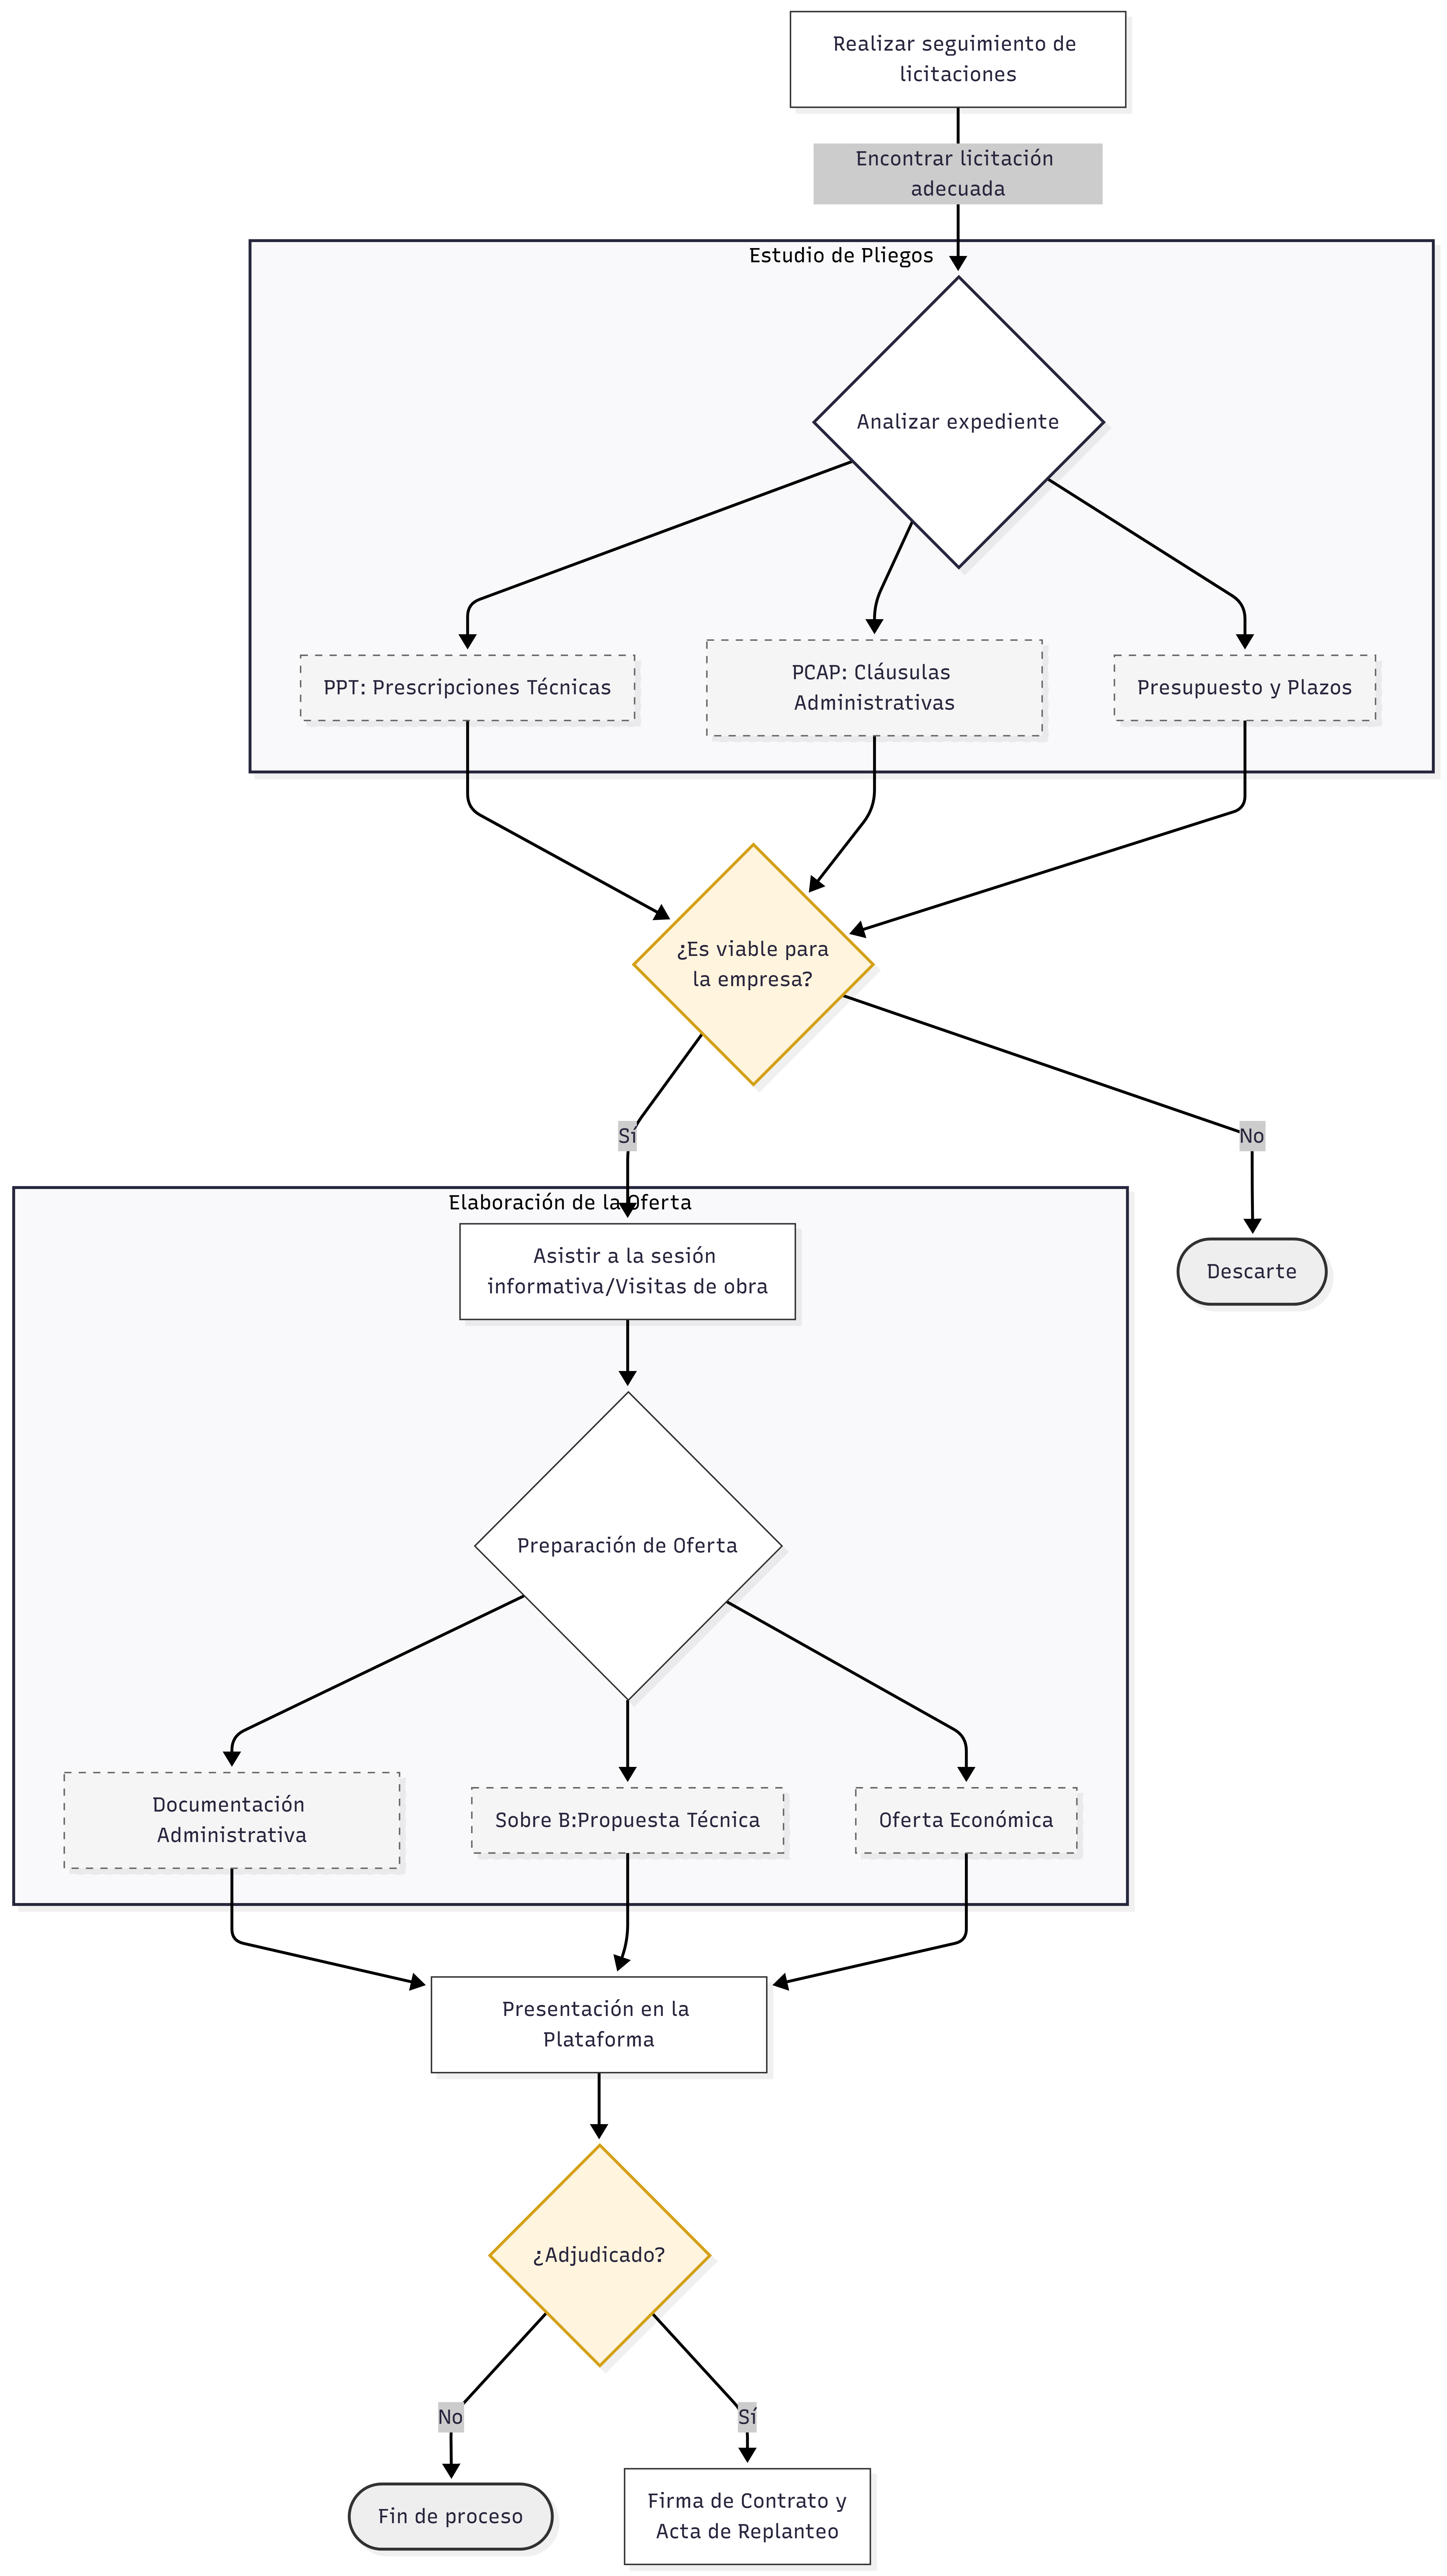
\includegraphics[width=0.65\textwidth]{figs/Procesos de licitación.png} 
    \caption{Diagrama de flujo del proceso de licitación}
    \label{fig:proceso_licitacion}
\end{figure}
\subsection{Marco administrativo y licitación pública}

\begin{figure}[ht]
    \centering
    \includegraphics[width=0.8\textwidth]{figs/construccion_aeropuerto.jpg}
    \caption{Obras de expansión en infraestructura aeroportuaria. Fuente: Olaf Tausch vía Wikimedia Commons (Licencia CC BY-SA 3.0).}
    \label{fig:construccion_aeropuerto}
\end{figure}
El canal principal en el cual poder encontar licitaciones públicas es la \textit{Plataforma de Contratación del Sector Público}, en la cual, diversas administraciones públicas ofertán un proyecto. Cuando se pública una licitación, es procesada como un \textbf{expediente} administrativo.
Cada expediente representa un proyecto licitado por la administración y se identifica mediante un número de identificación único. Este registro contiene información importante, tal como la fecha límite de presentación, el importe base de licitación, la descripción técnica y, fundamentalmente, el \textbf{pliego}. Este documento detalla las actuaciones a realizar y los requisitos técnicos y legales que la empresa debe cumplir para ser considerada apta.
Tras haber comentado los activos principales,se explicará la fase de busqueda de expedientes desde el punto de vista de las empresas. Las empresas analizan detalladamente el pliego para evaluar la viabilidad del proyecto, comprobando las actuaciones requeridas, la rentabilidad económica y los plazos de presentación. Si estas condiciones se ajustan a la capacidad e intereses de la entidad jurídica, se procede con la preparación de la oferta.
Para preparar la oferta, se deberá de recopilar cierta información, las empresas suelen obtenerla a través de la \textbf{presentación} del expediente, junto con visitas a la obra. Después de haber preparado la oferta, la cual contendrá una extensa documentación administrativa, junto con la oferta económica detallada para cada actuación descrita en el pliego, la administración publicadora evaluará todas las ofertas, y seleccionarán la mejor. Finalmente, en ese momento, podemos decir que la licitación ha sido\textbf{adjudicada}.
\subsection{Gestiones administrativas en entornos aeroportuarios}
Una vez adjudicada la obra, las labores en el recinto aeroportuario presentan diversas complicaciones, que se deben a las nomativas europeas \cite{UE_139_2014} las cuales fueron definidas por la Agencia Estatal de Seguridad Aérea (AESA) \cite{AESA_Web}. AESA actúa como el organismo regulador de la seguridad aérea en España, mientras que AENA ejerce como gestor, siendo los responsables del cumplimiento.
Los técnicos deben realizar reformas, junto con instalaciones eléctricas entre las que se incluyen las instalaciones de climatización en zonas de tránsito de pasajeros o \bft{áreas restringidas} (denominadas lado aire y lado tierra). Esto implica una serie de precauciones críticas que deben ser tratadas:
\begin{itemize}
\item{Formación Obligatoria:} Los trabajadores deben superar programas de formación específica. El curso AVSEC les capacita en la protección contra actos de interferencia ilícita \cite{AENA_AVSEC}, mientras que el AVSAF se centra en la seguridad operacional en pista \cite{AENA_AVSAF}. Sin estas certificaciones vigentes, el trabajador tiene denegado el acceso autónomo, dependiendo de acompañamiento autorizado, lo que penaliza la productividad.
\item{Logística de Accesos:} El transporte de materiales debe coordinarse con los horarios de baja operativa del aeropuerto, requiriendo escoltas o pases de seguridad temporales cuya gestión esta regida por reglas inflexibles, lo que provoca un retraso considerable.
\item{Gestión de Residuos:} El desescombro y la limpieza deben ser inmediatos y bajo normativas ambientales estrictas para no afectar a la calidad del aire o la visibilidad en terminales.
\end{itemize}
\begin{figure}[ht]
    \centering
    \includegraphics[width=0.8\textwidth]{figs/Tecnicos.jpg} 
    \caption{Operarios coordinando tareas de mantenimiento e infraestructura. Fuente: \textit{“Discussing the work”} por Oregon Department of Transportation, utilizada bajo licencia CC BY 2.0 (\url{https://creativecommons.org/licenses/by/2.0/}).}
    \label{fig:discusion_obra}
\end{figure}
\newpage
\section{Entorno digital del sector}
Una vez expuesto el marco administrativo y operativo al que se exponen las pequeñas y medianas empresas en la obra pública aeroportuaria, es de vital importancia analizar el entorno software con el que las empresas operan. En este apartado se evaluará el estado actual de digitalización del sector, identificando las carencias de las soluciones de las organizaciones y analizando las herramientas y aplicaciones que predominan actualmente en el mercado.
\subsection{Deuda técnica del sector}
A pesar de que el sector público ha avanzado hacia la administración electrónica, la digitalización en las pymes de la construcción e instalaciones presenta una evolución muy irregular \cite{ONTSI_Pymes, DESI2026}. Esta disparidad genera lo que en Ingeniería del Software se conoce como \textbf{deuda técnica}. Esta deuda se produce por el coste de mantener soluciones de software limitadas, parches temporales o arquitecturas deficientes en lugar de invertir en un sistema escalable y bien diseñado.
En el caso de estas empresas, la deuda técnica no suele provenir de código mal escrito, sino por la falta de un software especializado. Al contar con un capital limitado, siempre surge el miedo de invertir en algo nuevo que no se sabe cual va a ser su rentabilidad.
\begin{table}[h]
\centering
\renewcommand{\arraystretch}{1.2}
\begin{tabular}{|l|c|c|c|}
\hline
\rowcolor{gray!20} \bft{Sector de Actividad (2022)} & \bft{Total (\%)} & \bft{Total > 10 (\%)} & \bft{Total micro (\%)} \\ \hline
Construcción & 59,9 & 75,4 & 58,7 \\ \hline
Act. Inmobiliarias y Administrativas & 67,1 & 81,1 & 66,4 \\ \hline
\end{tabular}
\caption{Valor de la dimensión equipamientos e infraestructuras por tamaño de empresa. Fuente: Elaboración propia a partir de datos del ONTSI (2023)}
\label{tab:datos_ontsi_construccion}
\end{table}
\subsection{Soluciones software del sector}
A la hora de hablar de las soluciones software del sector, no existe una única herramienta integral que cubra todas las necesidades de una empresa. Por lo tanto, se debe abordar el ecosistema desde una perspectiva fragmentada, categorizando las aplicaciones según el area en el que se use. En la actualidad, las pymes se estructuran en los siguientes bloques software que suelen estar incomunicados entre ellos.
\subsubsection{Plataformas de licitacion}
Las empresas están obligadas a utilizar portales externos como los de AENA o los de la Plataforma de Contratación del Estado. Estas plataformas han agilizado la administración de expedientes, tanto desde el punto de vista de la entidad publicadora, como de la entidad licitadora. Sin embargo, estas webs obligana realizar procesos manuales y redundantes hacía los sistemas internos de la empresa.
%CAPTURA DE AENA O DE LA PLATAFORMA DE CONTRATACIÓN DEL ESTADO
\subsubsection{Gestión económica y facturación}
Para el cumplimiento fiscal y la contabilidad, las pymes recurren a software especializado. El principal inconveniente de estas soluciones en las pymes es que, aunque resuelven la parte administrativa, suelen quedar aisladas del resto de los procesos operativos técnicos de la obra. 
%CAPTURA FACTUSOL
Es importante destacar que este entorno va a cambiar con la inminente implantación del sistema \textbf{VeriFactu}. Impulsado por la Agencia Tributaria (AEAT) como medida antifraude, VeriFactu es un nuevo reglamento que exigirá que los programas informáticos de facturación garanticen la inalterabilidad, trazabilidad y conservación de los registros. Esto significa que el software deberá ser capaz de certificar las facturas y enviarlas automáticamente a la administración en tiempo real. 
Dado que Verifactu establece la normativa, las aplicaciones de facturación deberán adaptar su arquitectura para cumplir con las reglas impuestas. Aquellas herramientas que, por limitaciones o código heredado, no sean capaces de integrar las exigencias, quedarán obsoletas y saldrán del mercado. Esta transición obligará a muchas pymes a adoptar una nueva tecnología, lo cual generará varios problemas derivados entre los que se encuentan la curva de aprendizaje y, por consiguiente, una migración masiva de datos para el nuevo programa.
%CAPTURA DE ALGUNA NORMATIVA DE VERIFACTU
\subsubsection{Herramientas de gestión y almacenamiento de datos}
Ante la falta de sistemas centralizados, existe una tendencia generalizada en el sector a utilizar hojas de cálculo (principalmente Microsoft Excel) como herramientas principales para la gestión y almacenamiento de datos. Estos documentos asumen roles para los que no fueron diseñados, actuando como bases de datos improvisadas para el control de presupuestos, certificaciones de obra, inventario de materiales e incluso gestión de combustibles. 
Desde el punto de vista de la ingeniería del software, esta práctica genera una importante deuda técnica. Las hojas de cálculo carecen de propiedades transaccionales, no imponen restricciones de integridad referencial y presentan graves limitaciones en entornos de trabajo colaborativo o concurrente. La ausencia de un modelo de datos estructurado provoca duplicidad de información y dificulta la extracción de métricas fiables sobre el estado real de los proyectos.
%CAPTURA DE EXCEL
\subsubsection{Sistemas integrados de gestión (ERP)}
Por último, al analizar las soluciones tecnológicas del mercado, es inevitable mencionar los sistemas empresariales monolíticos, concretamente los sistemas de planificación de recursos empresariales (ERP, por sus siglas en inglés). 

En teoría, la implantación de un ERP resolvería el problema de la fragmentación de datos mencionado anteriormente, al unificar la facturación, los recursos humanos y la gestión de proyectos en una única plataforma. Sin embargo, en la práctica, estas soluciones presentan barreras de entrada críticas para las pymes del sector aeroportuario. Por un lado, suponen un coste económico y un tiempo de implantación inasumibles para empresas de tamaño reducido. Por otro lado, su arquitectura suele ser demasiado rígida para adaptarse a las particularidades y flujos de trabajo tan específicos que imponen organismos como AENA.

Por un lado, destacan los \textbf{ERPs genéricos y modulares}, entre los cuales podemos destacar Odoo, siendo una de las opciones mas valroadas por la pymes al ser Open Source. Permite a la empresa instalar únicamente las aplicaciones que necesitan. Además de Odoo, tambien existe Microsfot 365 Business central. Es el estandar corporativo,siendo robusto, pero presentando ciertas limitaciones, las principales serían sus licencias de alto coste, curva de aprendizaje y tiempos de de implantación que suelen ser meses.
%CAPTURA DE LOS ERPS
Por otro lado, existen \textbf{ERPs verticales específicos para la construcción}. Estos ERPs son soluciones diseñadas para el secotr de la construcción. Cuenta con modulos para hacer multiples gestiones como presupuestos o certificaciones de obra. De entras estas, podemos destacar Sigrid y BrickControl
%CAPTURA DE LOS ERPS
A pesar de la existencia de la existencia de estas potentes herramientas en el mercado, su adopción para empresas pequeñas es baja al presentar una arquitectura rígida que complica la adaptación a flujos de trabajo específicos. %Seguir, con el porque de que no se implemente en las pymes.
 

% Utilidades para anotaciones
\chapter{Propuesta de Solución, Metodología y Herramientas}
En este capítulo se aborda una descripción de la propuesta de solución, así como la descripción de la metodología utilizada a lo largo de este proyecto, junto con la adaptación que se ha llevado a cabo de esta.
Además, se menciona las herramientas que han sido utilizadas tanto para la gestión, desarrollo y documentación del proyecto.
\section{Propuesta de Solución}
Una vez adentrados en el contexto del sector y habiendo analizado algunas de las diversas aplicaciones que se suele emplear por la competencia, me propongo a realizar una descripción de la propuesta de solución para el desarrollo de este proyecto. Sin embargo, no he llegado a esta solución de manera inmediata, antes de la idea final he tenido más ideas que tras probarlas y analizarlas han sido descartadas.
\subsection{Primeras ideas}

\subsubsection{Primera Solucion}
Tras terminar el primer año pensé en migrar los datos de los diferentes proyectos a una base de datos en Access ¿Porque Access? al ser una aplicación de Microsoft 365 tiene una compatibilidad muy alta con Excel. En la \ref{fig:motivacion_Idea1} podemos ver un resumen de en que consistiría el proyecto. El problema fue que como he comentado anteriormente, había una diferencia muy grande entre los tipos de datos, como por ejemplo que en cada Excel la fecha se escriba de una forma, o que existan campos en algunas hojas que no vuelvan a aparecer en otras, por lo que habría que tomar una decisión importante en el diseño de la base de datos que se repetiría varias veces con distintos campos. Por lo tanto, al ver que la complejidad del proceso era cada vez mayor, decidí abandonar esta idea.
\begin{figure}[h]
    \centering
    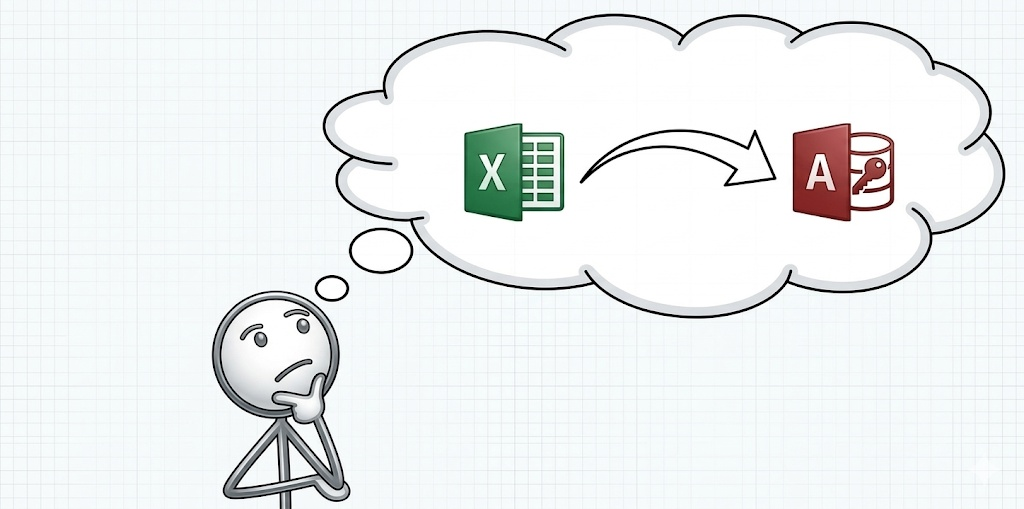
\includegraphics[width=0.7\textwidth]{figs/Primera_Idea.jpg}
    \caption{Ilustración conceptual de la primera solución propuesta.}
    \label{fig:motivacion_Idea1}
\end{figure}
\subsubsection{Segunda Solucion} 
Después del fracaso del pensamiento anterior, pensé en hacer un programa básico en Python que permitiese manejar varios procesos, es decir, una aplicación en miniatura, solo implementando el back y unas ayudas para que un usuario que no esté especializado pueda usarlo. Estas acciones irían desde un análisis de billetes de avión para ver cuál es más barato, para después poder comprar el seleccionado usando jsons con la información de los empleados que vayan a embarcar. En la \ref{fig:motivacion_Idea2} podemos ver un resumen de en que consistiría el proyecto.  
\begin{figure}[h]
    \centering
    \includegraphics[width=0.7\textwidth]{figs/Segunda_Idea.jpg}
    \caption{Ilustración conceptual de la segunda solución propuesta.}
    \label{fig:motivacion_Idea2}
\end{figure} 
Sin embargo, al igual que en el intento anterior cuanto más avanzaba con la idea, más contras salían, por decir algunas puedo nombrar la cantidad de llamadas que tendría que hacer a APIS de las páginas de las compañías de vuelos, junto con el mantenimiento masivo que tendría que hacer al intentar robotizar los formularios de los billetes de los aviones, esto debido a que los elementos html de estas webs son dinámicos.
\subsubsection{Conclusión}
Tras analizar las dos ideas, pensar como poder implementarlas juntas, analizando que pros y que contras tienen, todo esto con el fin de crear un producto con la mayor calidad posible. Pero tras darle un par de vueltas pensé en descartar las dos ideas y empezar algo nuevo, en vez de programar un programa básico en Python o unificar todos los datos. Porque no enfrentar primero cada problema por separado, primero, solucionar los procesos repetitivos a través de automatizaciones, como rellenar hojas de cálculo con un solo fichero de entrada, después ir construyendo una aplicación que contenga funciones más complejas como tableros Kanban para mejorar la autogestión entre otras, planings semanales para cada persona, sistema de fichado, entre otros. En la \ref{fig:motivacion_Idea3} podemos ver un prototipo de la idea.
\begin{figure}[h]
    \centering
    \includegraphics[width=0.7\textwidth]{figs/Conclusion_Idea.jpg}
    \caption{Ilustración conceptual de la idea del TFG.}
    \label{fig:motivacion_Idea3}
\end{figure}
\subsection{Automatizaciones posibles}
La identificación de procesos repetitivos permite proponer áreas de optimización mediante técnicas de automatización y orquestación de flujos \cite{IBMAutomation2024, EmprendeAprendiendo2025}. Se destacan la sincronización automática de datos de pases aeroportuarios y la monitorización de nuevas licitaciones mediante el consumo de fuentes oficiales y APIs.

\section{Tecnologías del sector}
El desarrollo de soluciones de gestión modernas requiere el análisis de paradigmas tecnológicos actuales que permitan superar la rigidez de los sistemas tradicionales. En esta sección se evalúan las tecnologías seleccionadas para la arquitectura del proyecto basándose en su rendimiento y fiabilidad en entornos profesionales \cite{Fowler2004, NodeJS_Official}.

\subsection{Arquitectura de Automatización y Datos}
Para integrar sistemas heterogéneos y garantizar la persistencia, se han analizado las siguientes categorías:
\begin{itemize}
    \item \textbf{Motores de Automatización:} Se evaluó el uso de scripts aislados frente a orquestadores visuales como \textit{n8n}, seleccionando este último por su capacidad de integración vía APIs y facilidad de mantenimiento \cite{IBMAutomation2024}.
    \item \textbf{Gestión de Bases de Datos:} Se compararon modelos NoSQL frente a Relacionales \cite{EDteamSQL, PandoraFMS_BD, MongoDB_Official}, optando por \textit{PostgreSQL} para asegurar la integridad referencial de los expedientes y certificaciones \cite{PostgreSQL_Official, TodoPostgreSQL_Ventajas}.
\end{itemize}

\subsection{Ecosistema de Desarrollo Full-Stack}
La creación de interfaces dinámicas como tableros Kanban requiere frameworks modernos. Se analizaron opciones como Angular y Vue \cite{Angular_Official, VueJS_Official}, seleccionando \textit{React} ya que es un estandar muy usado actualmente, eficiente y además he tenido la oportunidad de trabajar con él \cite{4GeeksFrameworks, React_Official, Vid_React_Tutorial}. En el servidor, se utiliza \textit{Node.js} con \textit{Express} para gestionar la asincronía de las tareas de automatización de forma eficiente \cite{NodeJS_Official, Express_Official}. Se podría utilizar springBoot que es más solido, pero no estoy familiarizado con él, mientras que Node es más facil de implementar y tengo algo de experiencia.

\section{Conclusiones de las Tecnologías}
Tras analizar el estado actual de las pymes del sector, se concluye que la superación de la deuda tecnológica requiere abandonar el modelo de silos manuales.
Por ultimo, gracias a una encuesta de \cite{StackOverflow2025} podemos observa cuanto usan los desarrolladores las tecnologías mencionadas.
\begin{figure}[h]
    \centering
    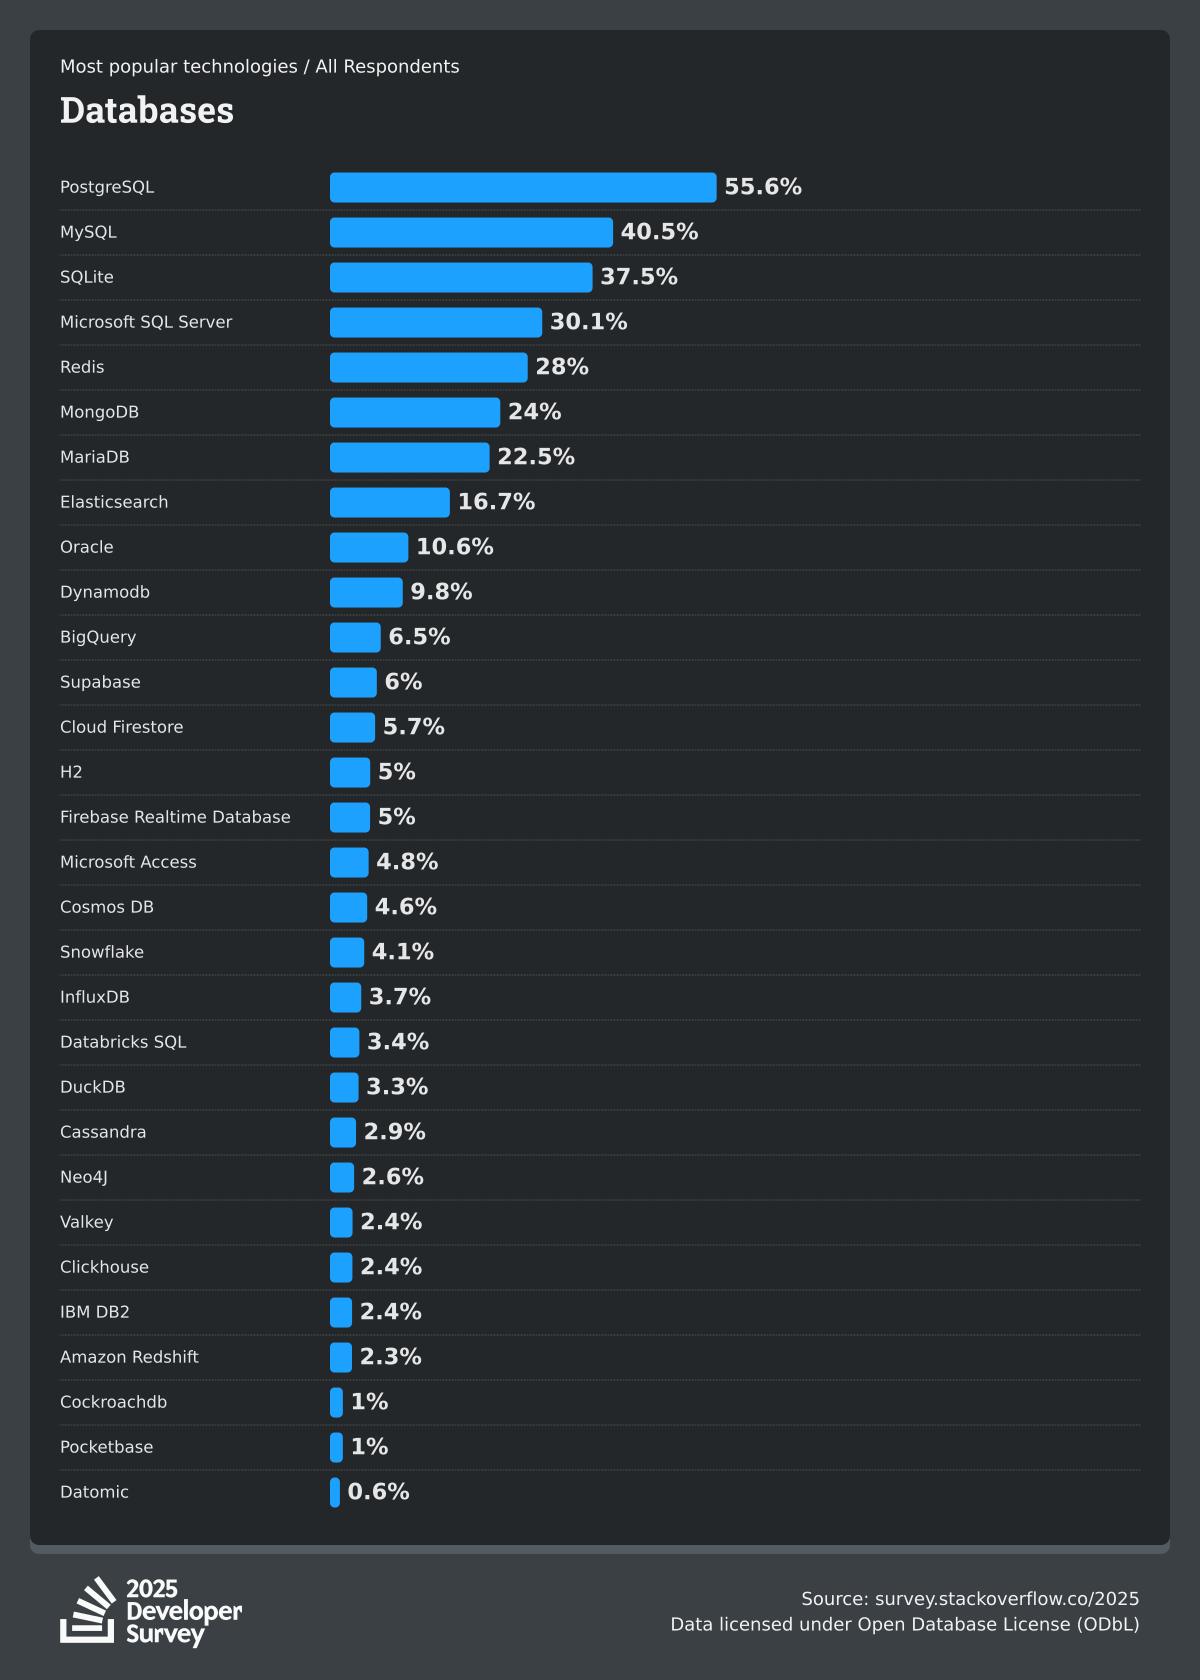
\includegraphics[width=0.8\textwidth]{figs/Databases_MasUsadas.png}
    \caption{Ilustración de las bases de datos más usadas. Fuente: \cite{StackOverflow2025}.}
    \label{fig:iceberg_deuda_tecnologica}
\end{figure}
\begin{figure}[h]
    \centering
    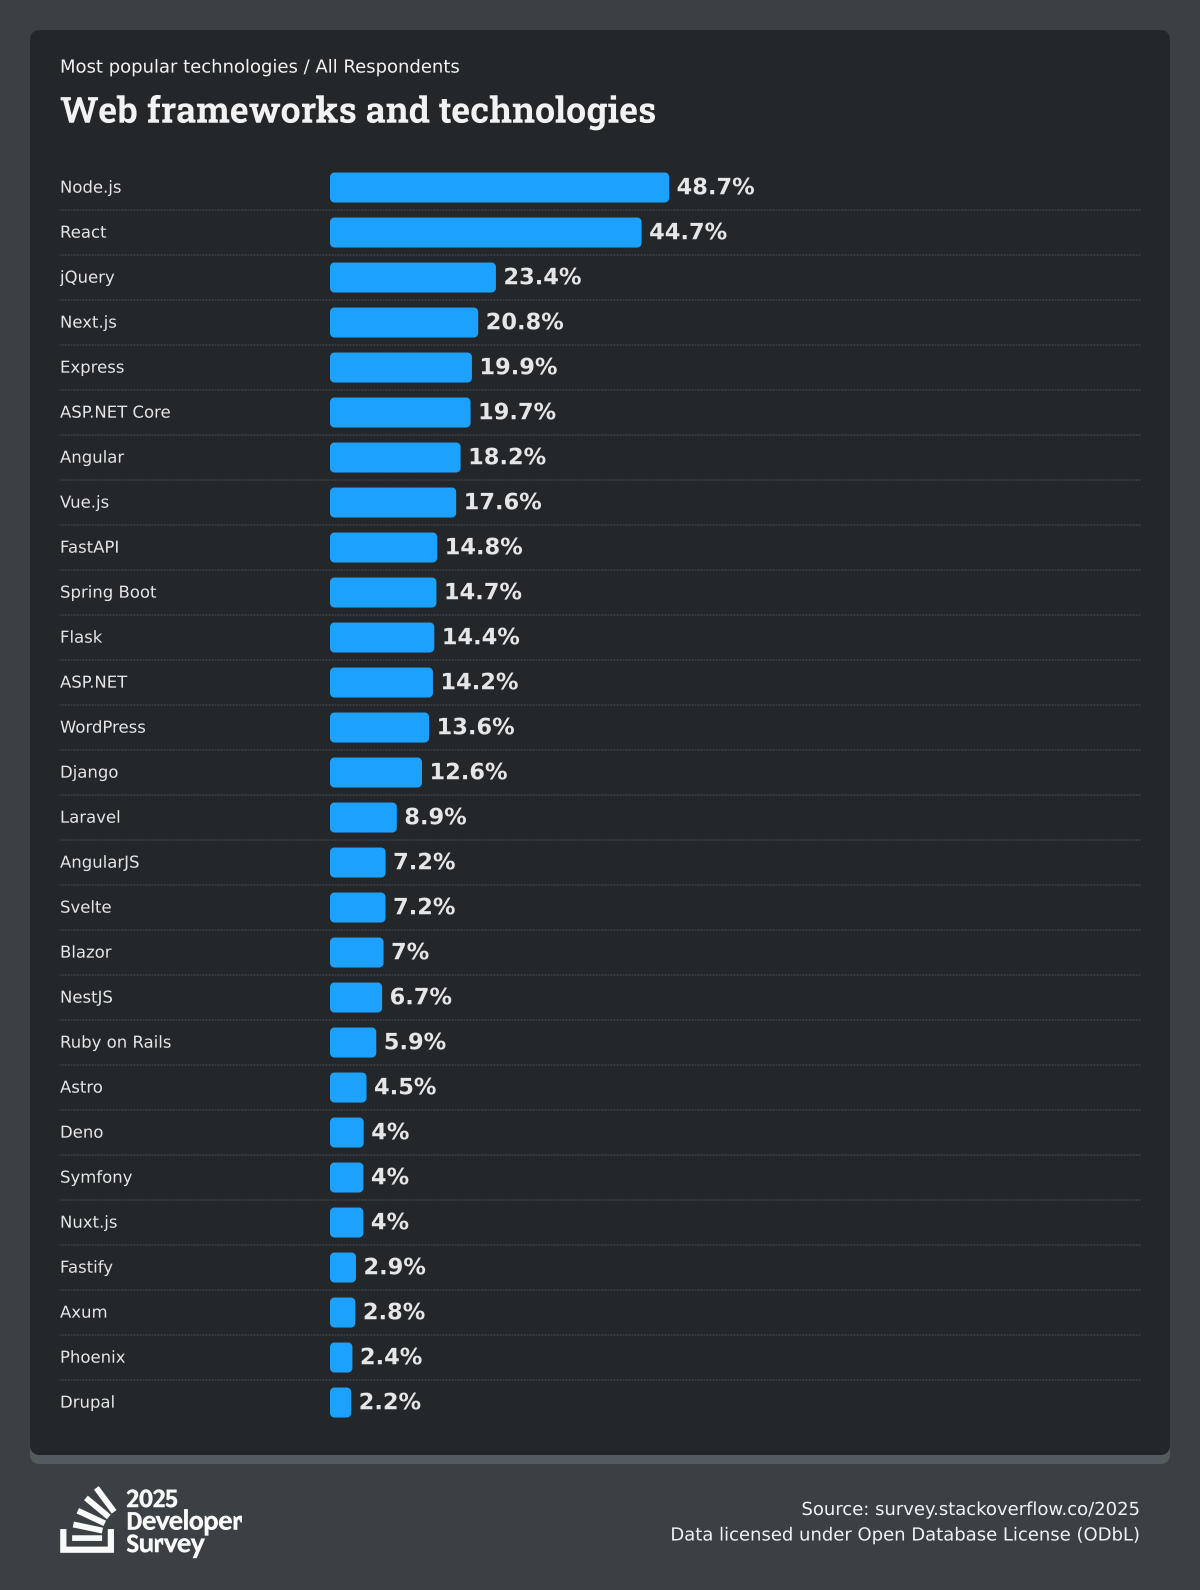
\includegraphics[width=0.8\textwidth]{figs/Frameworks_MasUsados.png}
    \caption{Ilustración de los frameworks más usados. Fuente: \cite{StackOverflow2025}.}
    \label{fig:iceberg_deuda_tecnologica}
\end{figure} 

% -------------------------------
% Apéndices
% -------------------------------
\appendix
\chapter{Tecnologías y Arquitectura de la Solución}
\label{ap:tecnologias}
\section{Automatizaciones}

La automatización de procesos de negocio consiste en el uso de la tecnología para ejecutar tareas y flujos de trabajo recurrentes, minimizando la intervención humana. En el contexto de la Ingeniería del Software, esto implica organizar diferentes sistemas, APIs y bases de datos para que la información fluya de manera autónoma en respuesta a eventos específicos que actuarán como disparadores o triggers.

Tras saber qué es una automatización, a continuación se detallan los tipos de automatizaciones que existen.

\subsection{Tipos de Automatizaciones}

Actualmente existen varios tipos de automatizaciones, cada tipo se enfoca en resolver un tipo de necesidad empresarial:

\begin{itemize}

    \item RPA (Automatizaciones robotizadas): Se centra en construir robots para interactuar con elementos de interfaces de usuario (UI) de la misma forma en la que lo haría un humano, ya sea haciendo clics, rellenando formularios, etc. Es útil para conectar servicios que cambian ante el mismo elemento, pero es muy frágil ya que los elementos de las webs suelen ser difíciles de seleccionar al tener identificadores dinámicos. Algunos de estos son Microsoft Power Automate Desktop o UiPath.

    \item Automatizaciones basadas en código: Consiste en programar scripts o procesos en segundo plano utilizando herramientas del propio lenguaje de programación (como Celery en Python o BullMQ en Node.js). Ofrece un control absoluto a nivel de arquitectura, pero carece de interfaces visuales para que un usuario no técnico entienda el flujo.

    \item Motores de Orquestación BPMN (Business Process Model and Notation): Plataformas empresariales complejas (como Camunda) que utilizan estándares formales para modelar y ejecutar procesos de negocio largos e intrincados. Están diseñadas para grandes corporaciones con flujos de aprobación de múltiples niveles. UiPath a parte de ser un motor de RPA, también ofrece un motor de orquestación BPMN, pero su complejidad y coste lo hacen poco adecuado para pymes.

    \item iPaaS y Motores de Flujo de Trabajo Visuales: Plataformas de integración como servicio (como n8n, Zapier o Make). Permiten conectar aplicaciones a través de sus APIs utilizando interfaces gráficas basadas en nodos. Son ágiles, escalables y perfectas para reaccionar a eventos web en tiempo real.

\end{itemize}

\subsection{Herramienta elegida}

Tras esta investigación sobre todos los tipos de herramientas posibles para automatizar, se han evaluado las diferentes alternativas y se ha determinado que la mejor para implementar en este proyecto es n8n. 

Se ha elegido esta sobre las demás ya que, al ser una herramienta fair-code, permite desplegarla en cualquier infraestructura, ya sea mediante Docker o mediante instalación directa. Además de esto, permite poner en práctica la competencia IS3[cite: 16], la cual consiste en dar solución a problemas de integración entre tecnologías. Por último, permitirá integrarse con la aplicación principal a través de llamadas de API, a diferencia de herramientas como Power Automate o UiPath que funcionan como aplicaciones aisladas.

\section{Base de Datos}

Para el correcto funcionamiento de la aplicación, es fundamental seleccionar un sistema de almacenamiento de datos que se adapte a las necesidades del proyecto. Este sistema deberá gestionar el registro tanto de empresas como de particulares, así como la información relativa a las obras e instalaciones, incluyendo la creación de ítems, la gestión de tareas y la visualización de su estado de forma estructurada. Como parte de la evaluación de distintas tecnologías para implementar la arquitectura de la solución, a continuación se analizan los principales modelos de bases de datos y sus opciones de alojamiento.

\subsection{Modelo de base de datos}

A la hora de estructurar y almacenar la información, existen dos paradigmas principales en la industria del software:

\begin{itemize}
    \item \textbf{Bases de Datos Relacionales (SQL):} Este modelo almacena la información en tablas estrictas compuestas por filas y columnas, estableciendo relaciones claras entre ellas mediante claves primarias y foráneas. Garantizan la integridad referencial y son ideales para dominios de datos altamente estructurados, como la relación entre un usuario, su empresa y sus tareas asignadas. Las bases de datos más famosas y utilizadas en este ámbito son PostgreSQL, MySQL, MariaDB y Oracle Database.

    \item \textbf{Bases de Datos No Relacionales (NoSQL):} Este paradigma prescinde de esquemas fijos y tablas, almacenando la información en formatos más flexibles como documentos, grafos o pares clave-valor. Son altamente escalables y útiles cuando la estructura de los datos es cambiante o impredecible. Los ejemplos más destacados de bases de datos NoSQL incluyen MongoDB, Cassandra, Redis y CouchDB.
\end{itemize}

Para contextualizar el uso de estas tecnologías en el mercado actual, la Figura \ref{fig:so_databases} muestra los resultados de la encuesta anual de desarrolladores de Stack Overflow, evidenciando la consolidación de PostgreSQL como el sistema de gestión de bases de datos más utilizado y deseado por los profesionales.

\begin{figure}[ht]
    \centering
    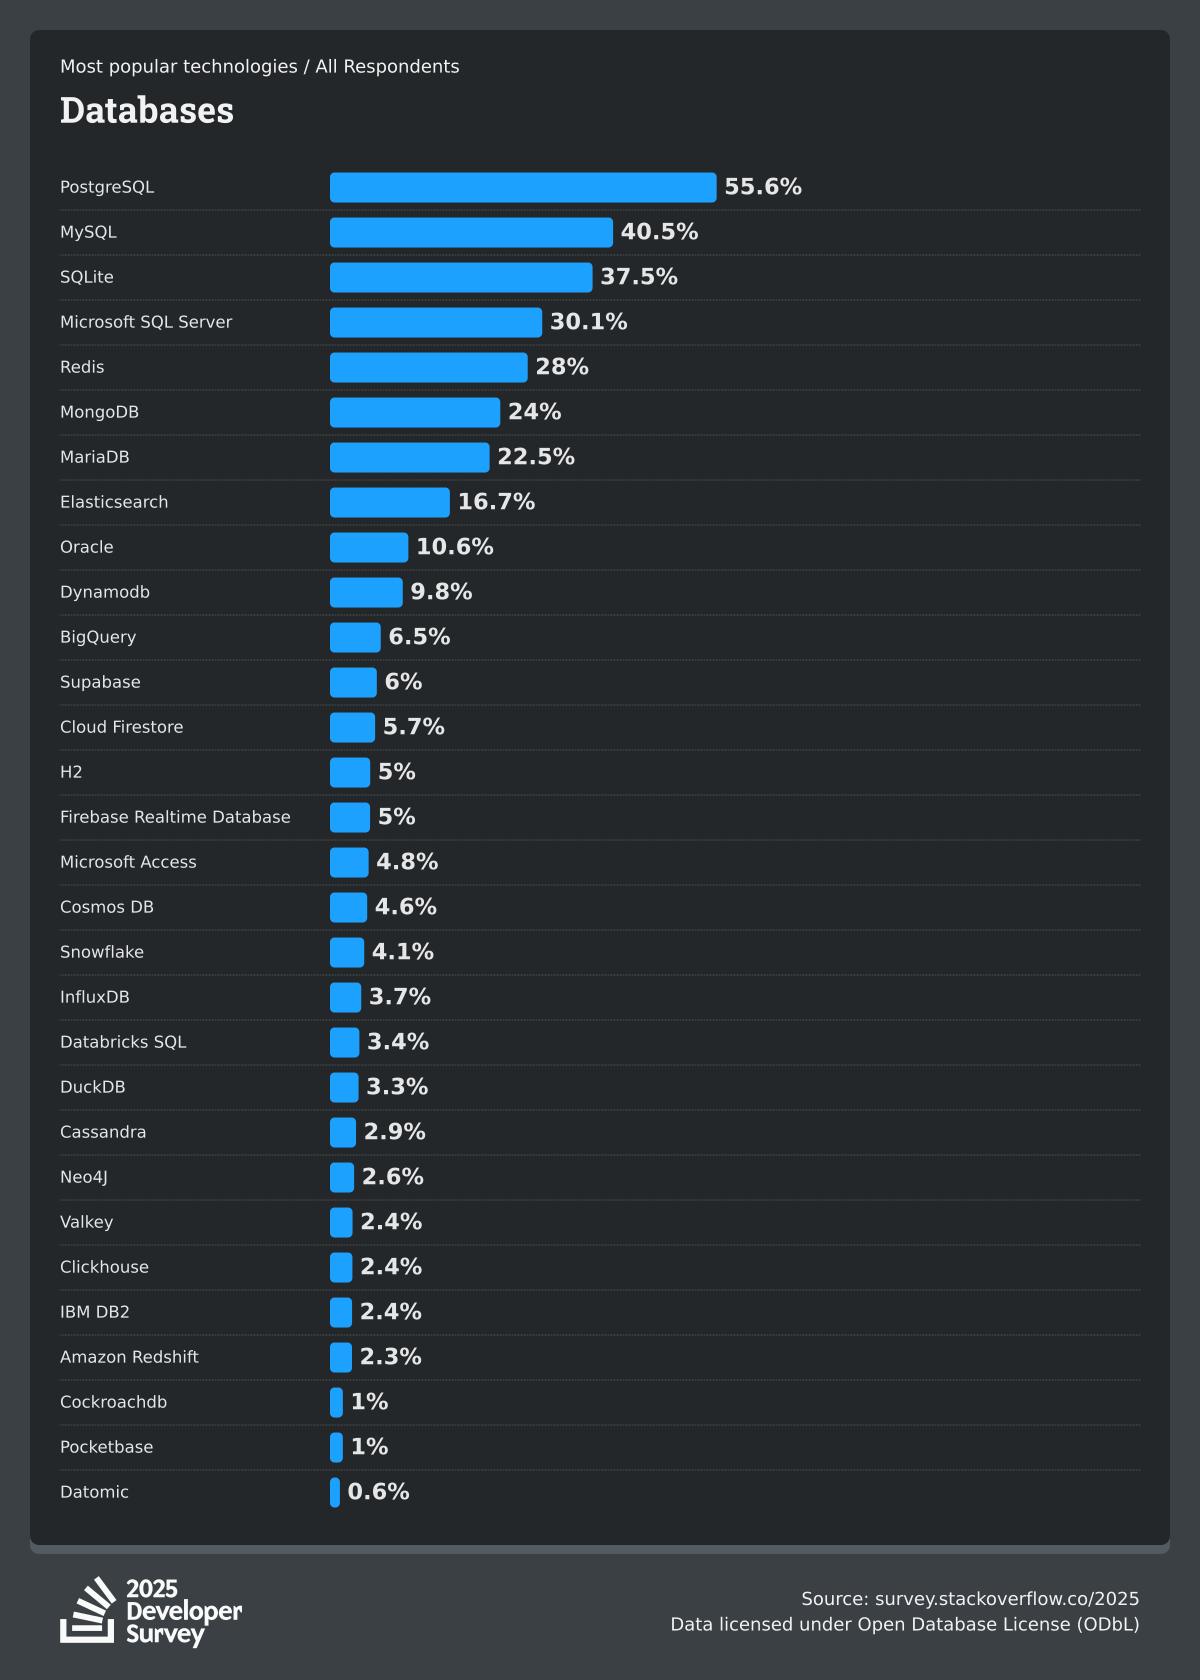
\includegraphics[width=0.8\textwidth]{figs/Databases_MasUsadas.png}
    \caption{Bases de datos más populares según la encuesta anual de Stack Overflow. Fuente: \cite{StackOverflow2025}.}
    \label{fig:so_databases}
\end{figure}

\subsection{Alojamiento}

Una vez definido el modelo de datos, es necesario determinar dónde y cómo se desplegará el motor de la base de datos, existiendo dos enfoques principales:

\begin{itemize}
    \item \textbf{Alojamiento en la Nube (Cloud / DBaaS):} También conocido como \textit{Database as a Service}, consiste en delegar la infraestructura, el mantenimiento y las copias de seguridad a un proveedor de servicios en la nube. Permite una alta disponibilidad sin necesidad de gestionar la infraestructura subyacente. Entre los servicios más famosos se encuentran Amazon RDS (AWS), Google Cloud SQL, MongoDB Atlas y plataformas modernas como Supabase o Firebase.

    \item \textbf{Alojamiento Local (On-Premise / Self-Hosted):} En este modelo, el motor de base de datos se instala y gestiona directamente en servidores propios o en la máquina local, frecuentemente utilizando tecnologías de contenerización. Ofrece un control absoluto sobre los datos, la configuración de red y la arquitectura, reduciendo la dependencia económica de terceros. Herramientas como Docker facilitan enormemente este tipo de despliegues estandarizados.
\end{itemize}

\subsection{Elección tecnológica}

Tras evaluar los diferentes modelos y opciones de alojamiento, se ha determinado que la tecnología de base de datos óptima para el desarrollo de esta aplicación es \textbf{PostgreSQL}, instalada y desplegada de manera local en la propia máquina (\textit{On-Premise}).

La elección de un modelo relacional como PostgreSQL se fundamenta en la naturaleza estructurada de la información que la aplicación debe manejar. Dado que el sistema permitirá al usuario registrar tanto una empresa como a un particular, y ofrecerá un tablero Kanban para crear ítems y gestionar tareas de forma clara y estructurada, es imperativo contar con la integridad referencial que proporciona una base de datos SQL para asegurar la consistencia entre las entidades.

Por otro lado, se opta por una instalación local debido a dos factores críticos para el proyecto:

\begin{itemize}
    \item \textbf{Facilidad de uso e implementación:} Alojar la base de datos en la propia máquina (utilizando tecnologías de contenerización como Docker) simplifica enormemente el entorno de desarrollo y permite implementar y evaluar la solución de forma rápida e independiente.
    \item \textbf{Seguridad y control de datos:} Mantener la base de datos en infraestructura propia garantiza un control absoluto sobre el acceso a la información. Al estar orientada a facilitar el funcionamiento de pequeñas y medianas empresas, es vital asegurar que sus datos operativos no se expongan innecesariamente a servicios de terceros, reforzando la privacidad y la fiabilidad del sistema.
\end{itemize}

\section{Frontend (Interfaz de Usuario)}

El Frontend constituye la capa de presentación de la aplicación, siendo el punto de interacción directo con el usuario. En el contexto de este proyecto, esta capa asume una responsabilidad crítica, ya que debe proporcionar una experiencia fluida tanto para el registro de empresas y particulares, como para la manipulación interactiva del tablero Kanban, permitiendo crear ítems, gestionar tareas y visualizar su estado de forma clara y estructurada.

A continuación, se analizan los paradigmas y tecnologías disponibles para el desarrollo de esta interfaz.

\subsection{Paradigmas de Arquitectura Web}

El desarrollo de interfaces web ha evolucionado significativamente, destacando dos enfoques principales en la actualidad:

\begin{itemize}
    \item \textbf{Multi-Page Application (MPA):} Es el modelo tradicional donde cada interacción del usuario con el servidor devuelve una página HTML completamente nueva. Aunque es excelente para el posicionamiento SEO (\textit{Search Engine Optimization}), resulta ineficiente para aplicaciones altamente interactivas, ya que las recargas constantes interrumpen la experiencia del usuario.
    
    \item \textbf{Single-Page Application (SPA):} En este modelo, el navegador carga un único documento HTML inicial y actualiza dinámicamente el contenido mediante JavaScript al interactuar con el backend a través de APIs. Este enfoque proporciona una fluidez similar a la de una aplicación de escritorio, siendo el estándar actual para herramientas de gestión e interfaces ricas.
\end{itemize}

\subsection{Tecnologías y Frameworks}

El desarrollo web moderno se asienta sobre lenguajes estándar de Internet como HTML, CSS y JavaScript. Sin embargo, para gestionar la complejidad de una SPA, la industria utiliza \textit{frameworks} y librerías que optimizan la manipulación del DOM (\textit{Document Object Model}):

\begin{itemize}
    \item \textbf{Angular:} Un \textit{framework} robusto y completo mantenido por Google. Impone una arquitectura estricta basada en TypeScript y el patrón Modelo-Vista-Controlador (MVC). Es ideal para proyectos empresariales a gran escala, pero posee una curva de aprendizaje pronunciada.
    
    \item \textbf{React:} Una librería desarrollada por Meta (Facebook) enfocada en la creación de interfaces de usuario mediante componentes reutilizables y un DOM virtual. Su ecosistema es inmenso y permite una gran flexibilidad arquitectónica.
    
    \item \textbf{Vue.js:} Un \textit{framework} progresivo que combina la robustez de Angular con la flexibilidad y simplicidad de React. Destaca por su curva de aprendizaje suave y su excelente documentación.
\end{itemize}

La adopción masiva de estas tecnologías queda reflejada en la encuesta a desarrolladores de Stack Overflow (Figura \ref{fig:so_frontend}), donde React destaca como la tecnología web más popular de la industria, superando a sus competidores directos y consolidando su posición como el estándar de facto para el desarrollo de interfaces modernas.

\begin{figure}[ht]
    \centering
    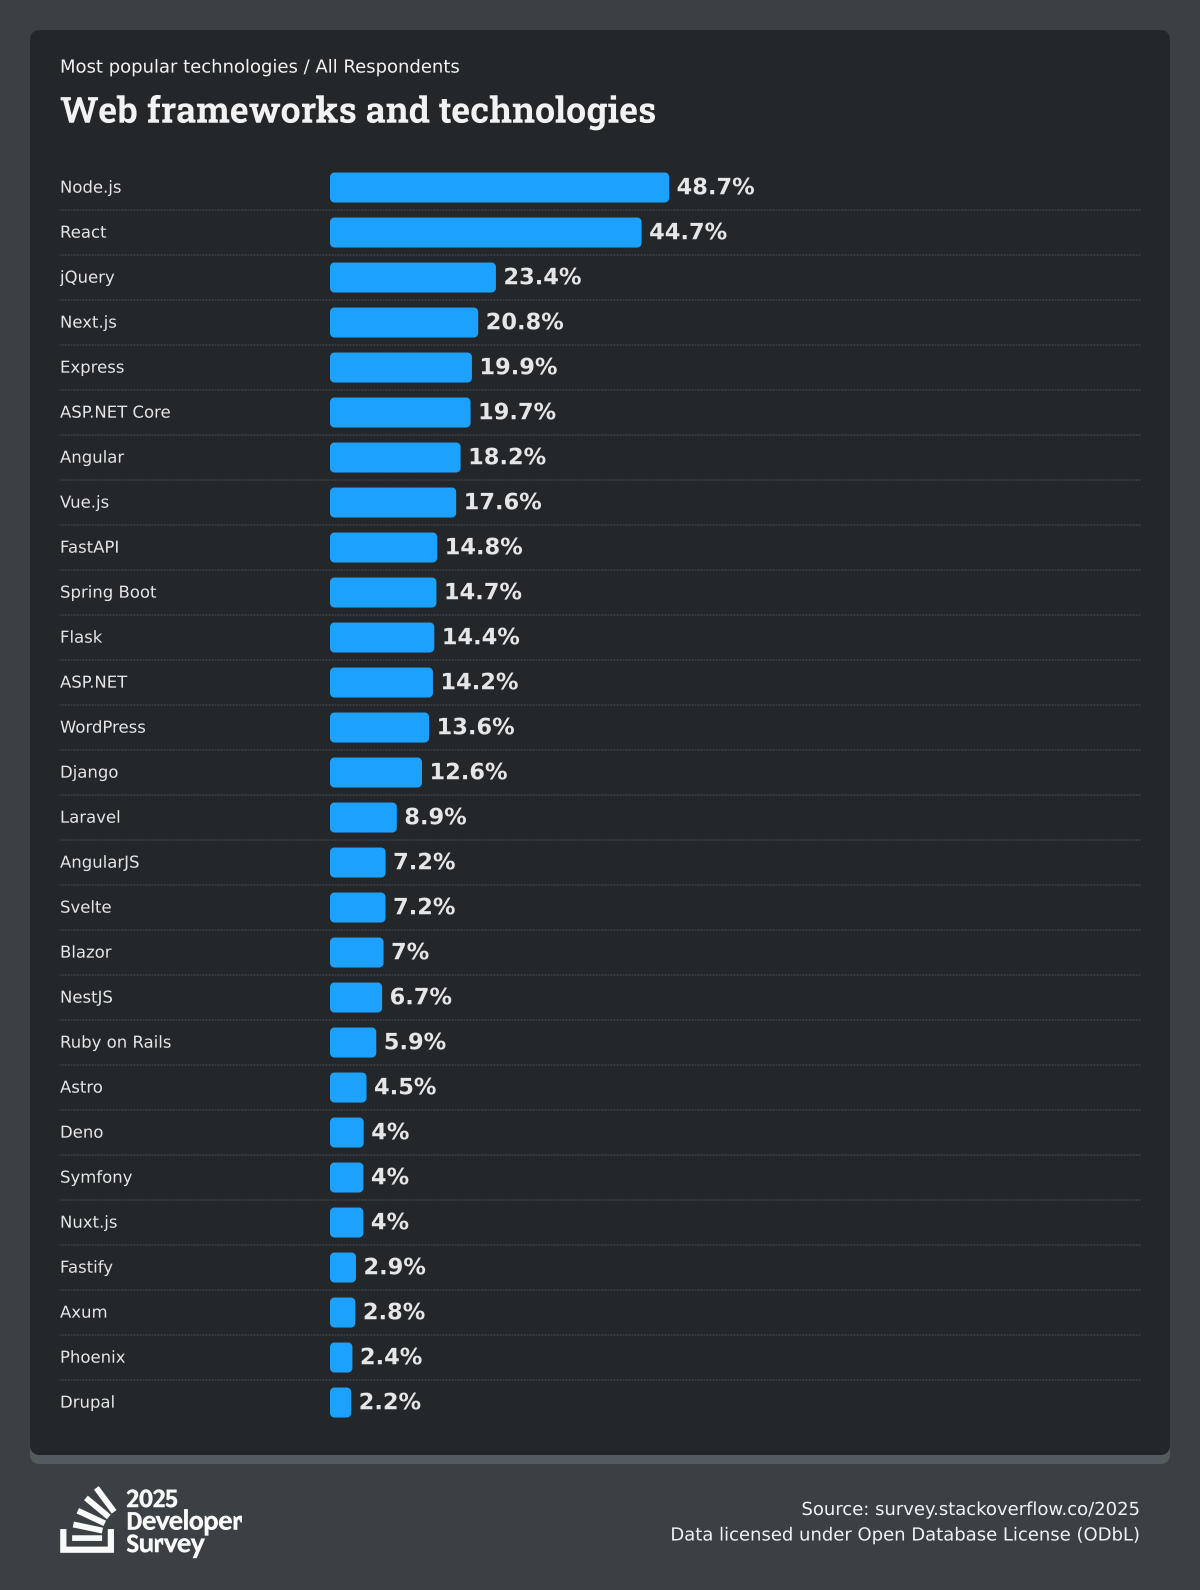
\includegraphics[width=0.8\textwidth]{figs/Frameworks_MasUsados.png}
    \caption{Frameworks web más populares según la encuesta anual de Stack Overflow. Fuente: \cite{StackOverflow2025}.}
    \label{fig:so_frontend}
\end{figure}

\subsection{Elección tecnológica}

Tras analizar los requisitos del sistema, se ha determinado que el desarrollo del Frontend se realizará con la librería \textbf{React} (junto con lenguajes estándar como JavaScript, HTML y CSS).

La justificación de esta elección se basa en los siguientes puntos:

\begin{itemize}
    \item \textbf{Arquitectura basada en componentes:} El requisito central de la interfaz es ofrecer un tablero Kanban que facilitará la organización y coordinación entre los usuarios. React permite encapsular la lógica y el diseño de cada "columna", "tarea" o "formulario de solicitud" en componentes independientes y reutilizables, aplicando principios sólidos de la Ingeniería del Software.
    
    \item \textbf{Gestión del estado e interactividad:} En un tablero Kanban, mover una tarea de una columna a otra requiere actualizar la interfaz en tiempo real sin recargar la página. El DOM virtual de React y su eficiente gestión del estado local garantizan una experiencia de usuario rápida y sin interrupciones visuales.
    
    \item \textbf{Ecosistema de librerías:} React cuenta con un extenso ecosistema de herramientas de código abierto, incluyendo librerías específicas para implementar funcionalidades de "arrastrar y soltar" (\textit{drag-and-drop}), las cuales son indispensables para el correcto funcionamiento del tablero de tareas.
\end{itemize}

\section{Backend (Lógica de Servidor y API)}

El Backend constituye la lógica central de la aplicación. Su responsabilidad principal es gestionar la autenticación de los usuarios, aplicar las reglas de negocio necesarias para el registro de empresas y particulares, e interactuar de forma segura con la base de datos PostgreSQL. Además, en esta arquitectura actuará como el orquestador principal que enviará y recibirá eventos hacia el motor de automatización n8n.

\subsection{Lenguajes y Entornos de Ejecución}

Para el desarrollo de la Interfaz de Programación de Aplicaciones (API), existen diversos entornos y lenguajes ampliamente adoptados en la industria de la Ingeniería del Software:

\begin{itemize}
    \item \textbf{Java (con Spring Boot):} Es el estándar empresarial por excelencia. Ofrece un tipado estricto, una máquina virtual muy madura y un marco de trabajo robusto que fomenta la aplicación de patrones de diseño clásicos. Aunque es excelente para sistemas corporativos de gran escala, su configuración inicial y verbosidad pueden resultar pesadas para un desarrollo ágil y rápido.
    \item \textbf{Python (con Django o FastAPI):} Python es un lenguaje altamente legible y versátil. Django ofrece una solución monolítica con "baterías incluidas" ideal para desarrollos rápidos, mientras que FastAPI destaca por su alto rendimiento y la autogeneración de documentación de APIs basada en estándares como OpenAPI. Sin embargo, esta opción aumenta la complejidad ya que necesita muchas dependencias externas para gestionar la asincronía y la integración con n8n.
    \item \textbf{Node.js (con Express o NestJS):} Permite ejecutar JavaScript (o TypeScript) del lado del servidor. Su arquitectura orientada a eventos y de entrada/salida asíncrona lo hace extremadamente eficiente para manejar múltiples peticiones concurrentes y llamadas a servicios externos. Se apoya fuertemente en formatos estándar de intercambio de datos de Internet como JSON.
\end{itemize}

\subsection{Elección tecnológica}

Como parte del objetivo de evaluar distintas tecnologías para implementar la arquitectura de la solución, se ha decidido desarrollar el Backend utilizando el entorno \textbf{Node.js}.

La elección de esta tecnología se fundamenta en las siguientes razones técnicas y metodológicas:

\begin{itemize}
    \item \textbf{Gestión de asincronía y Webhooks:} Dado que la aplicación delega la ejecución de procesos repetitivos a n8n, el servidor debe manejar eficientemente múltiples llamadas de red de forma asíncrona. Node.js está diseñado inherentemente para este tipo de cargas de trabajo no bloqueantes, garantizando que el sistema se comporte de forma fiable y eficiente.
    \item \textbf{Sinergia de lenguaje (Full-Stack JavaScript):} Al haber seleccionado un paradigma SPA (\textit{Single-Page Application}) para el Frontend, el uso de Node.js permite unificar el ecosistema en toda la pila tecnológica. Esto facilita el mantenimiento del código, el intercambio de estructuras de datos mediante JSON, y agiliza la resolución de las necesidades mínimas en cada \textit{sprint} de la metodología ágil adoptada.
    \item \textbf{Integración y escalabilidad:} El extenso ecosistema de paquetes de Node.js permite dar solución a problemas de integración de forma rápida, proporcionando herramientas maduras para la conexión con PostgreSQL, la gestión de autenticación y la comunicación con APIs de terceros.
\end{itemize}
\cleardoublepage
\thispagestyle{empty}
\chapter{Desarrollo del proyecto}
\section{Sprint 1: Investigación del sector e investigación tecnológica}
\subsection{Duración y objetivos del Sprint}
Durante este primer sprint, el objetivo principal fue realizar una investigación exhaustiva sobre las tecnologías más adecuadas para el proyecto y comprender el funcionamiento de los procesos de obra pública. Se evaluaron diferentes opciones de arquitectura, incluyendo motores de automatización, sistemas de bases de datos, frameworks de frontend y entornos de backend. En cuanto a la memoria, se buscó completar el capítulo 1 y 2 de la memoría, que son respectivamente la introducción y los antecedentes.
Este sprint se desarrolló desde el 19 de febrero de 2026 hasta el 18 de marzo de 2026, en un principio duraba 3 semanas, pero se extendió una semana más con el fin de dejar el primer y el segundo capítulo terminados.
\subsection{Desarrollo del Sprint}
En esta fase, el trabajo se centró en la exploración del ecosistema administrativo de las pymes que colaboran con empresas públicos como AENA. Se investigó el funcionamiento de la Plataforma de Contratación del Sector Público y los requisitos de gestión documental (planes de seguridad, certificaciones AVSEC/AVSAF) que generan la mayor carga administrativa.
Además, se realizó un análisis técnico comparativo para definir el stack tecnológico:
\begin{itemize}
    \item Para el Frontend, se evaluaron Angular, React y Vue.js, seleccionando React por su enfoque basado en componentes y su ecosistema de librerías para interfaces interactivas.
    \item Para el Backend, se compararon Java (Spring Boot), Python (Django/FastAPI) y Node.js (Express/NestJS), optando por Node.js debido a su eficiencia en la gestión de asincronía y su sinergia con el Frontend.
    \item Para la base de datos, se contrastaron modelos SQL y NoSQL, eligiendo PostgreSQL por su capacidad para garantizar la integridad referencial en un dominio de datos estructurado.
    \item Para la automatización, se analizaron RPA, scripts personalizados y motores de orquestación visual, decantándose por n8n por su flexibilidad y facilidad de integración mediante APIs.
\end{itemize}
\subsection{Reunión del sprint}
\subsection{Reunión de retrospectiva}
\begin{table}[H]
    \centering
    \caption{Resumen de estimación y esfuerzo real en Sprint 1.}
    \label{tab:esfuerzo_s1}
    \begin{tabular}{|c|c|c|}
        \hline
        \textbf{ID de Sprint} & \textbf{Estimación (Story Points)} & \textbf{Esfuerzo Real (Horas)} \\ \hline
        S1 & 38 & 45 \\ \hline % Valores de ejemplo basados en tu progreso
    \end{tabular}
\end{table}
\chapter{Diagramas y esquemas}
\section{Diagrama de procesos de licitación}
En este apartado se incluye la versión extendida y detallada del ciclo de vida de una licitación pública, simplificado previamente en la Figura \ref{fig:proceso_licitacion} del Capítulo 2. Este diagrama desglosa exhaustivamente las fases de estudio de pliegos, preparación de la oferta y adjudicación.
\begin{figure}[h]
    \centering
    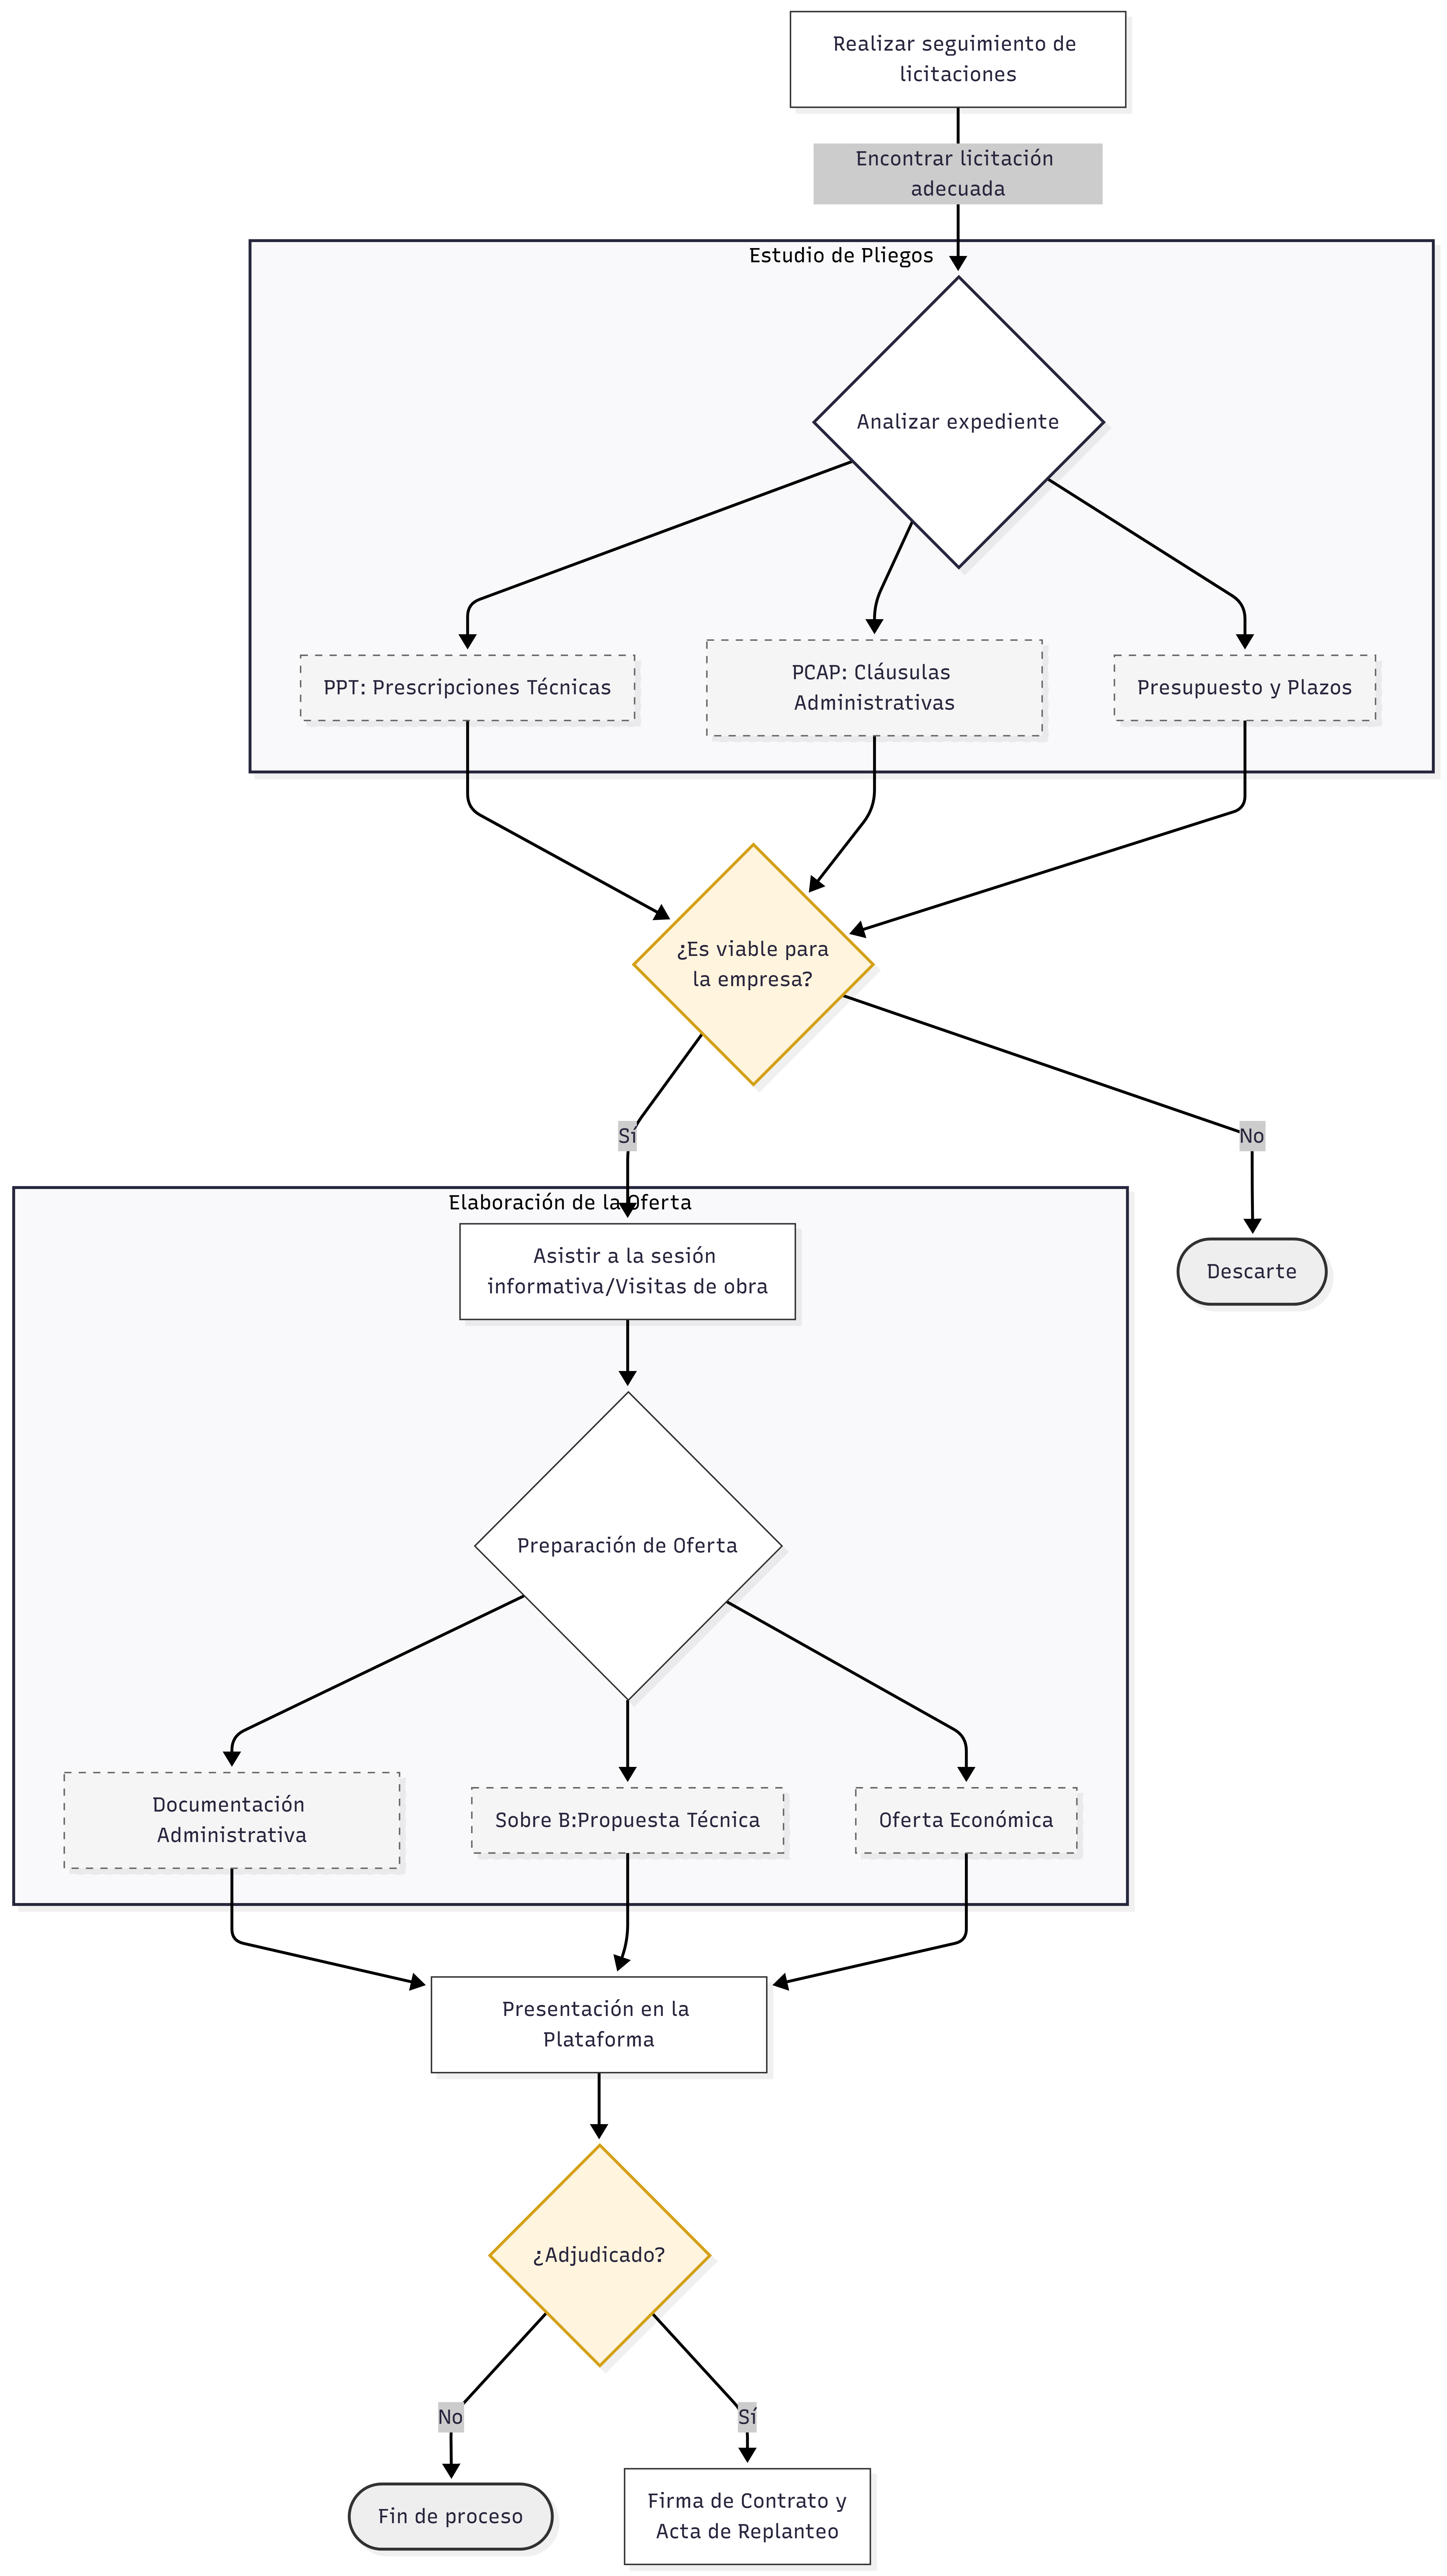
\includegraphics[width=0.8\textwidth]{figs/Procesos de licitación.png} 
    \caption{Diagrama de flujo detallado del proceso de licitación. Elaboración propia.}
    \label{fig:diagrama_completo}
\end{figure}
% -------------------------------
% Glosario
% -------------------------------
\chapter*{Glosario de Términos}
% La siguiente línea es para que el glosario aparezca en el Índice General
\addcontentsline{toc}{chapter}{Glosario de Términos}

A continuación, se definen los principales términos técnicos, acrónimos y conceptos administrativos utilizados a lo largo de este Trabajo de Fin de Grado para facilitar su comprensión:

\begin{description}
    \item[AENA] Aeropuertos Españoles y Navegación Aérea. Entidad pública empresarial encargada de la gestión de los aeropuertos de interés general en España.
    \item[AESA] Agencia Estatal de Seguridad Aérea. Organismo del Estado que vela por que se cumplan las normas de aviación civil.
    \item[API] (\textit{Application Programming Interface}). Conjunto de subrutinas, funciones y procedimientos que ofrece cierta biblioteca para ser utilizada por otro software como una capa de abstracción.
    \item[AVSAF] (\textit{Aviation Safety}). Certificación de seguridad operacional requerida para el personal que accede a la zona de movimiento de un aeropuerto.
    \item[AVSEC] (\textit{Aviation Security}). Certificación centrada en la protección de la aviación civil contra actos de interferencia ilícita.
    \item[PCAP] Pliego de Cláusulas Administrativas Particulares. Documento que rige los pactos y condiciones definidores de los derechos y obligaciones de las partes en un contrato público.
    \item[PPT] Pliego de Prescripciones Técnicas. Documento que contiene las especificaciones técnicas que han de regir la realización de la prestación objeto de una licitación.
    \item[RPA] (\textit{Robotic Process Automation}). Automatización robótica de procesos mediante el uso de software con inteligencia artificial y capacidades de aprendizaje automático para manejar tareas repetitivas de gran volumen.
    \item[Webhook] Callback HTTP definido por el usuario que se activa mediante un evento específico, utilizado para notificar a sistemas externos (como n8n) en tiempo real.
    \item[ERP] (\textit{Enterprise Resource Planning}). Sistema de planificación de recursos empresariales. Software monolítico que integra y automatiza las principales prácticas y procesos de negocio de una empresa (contabilidad, recursos humanos, inventario, etc.) en una única plataforma.
    \item[ONTSI] Observatorio Nacional de Tecnología y Sociedad de la Información. Órgano colegiado de carácter consultivo de la Administración General del Estado de España, fuente de los datos estadísticos sobre digitalización de las pymes.
    \item[Open Source] (Código abierto). Modelo de desarrollo de software basado en la colaboración abierta, donde el código fuente es accesible públicamente para que cualquiera pueda estudiarlo, modificarlo y distribuirlo.
    \item[Backend] (o Back-end). Capa de acceso a datos y lógica de negocio de una aplicación o sistema. Opera en el servidor, procesando la información y comunicándose con la base de datos, por lo que no es directamente visible para el usuario final.
    \item[Base de datos relacional] Tipo de base de datos que almacena y proporciona acceso a puntos de datos que están relacionados entre sí, organizando la información habitualmente en tablas compuestas por filas y columnas.
    \item[JSON] (\textit{JavaScript Object Notation}). Formato de texto ligero, estructurado y legible por humanos, utilizado como estándar para el intercambio de datos entre diferentes sistemas y lenguajes de programación.
    \item[Kanban] Marco de trabajo visual para la gestión ágil de proyectos. Utiliza tableros divididos en columnas (que representan fases del proceso) y tarjetas (que representan tareas) para optimizar el flujo de trabajo y evitar cuellos de botella.
    \item[Script] Archivo o fragmento de código que contiene una secuencia de comandos o instrucciones diseñadas para ser ejecutadas de forma automatizada por un programa interpretador, en lugar de ser compiladas.
    \item[Web Scraping] Técnica utilizada para extraer información y datos de sitios web de forma automatizada. Consiste en el uso de software que simula la navegación humana para leer y capturar el contenido del código HTML de las páginas.
\end{description}
% -------------------------------
% Bibliografía
% -------------------------------
\bibliographystyle{apalike}
\bibliography{bib/ref} 
\addcontentsline{toc}{chapter}{Referencia bibliográfica} % Añade a la tabla de contenidos

\end{document}